\documentclass[../homework.tex]{subfiles}
 \graphicspath{{\subfix{../images/}}}

\begin{document}

\section{Методика решения}


\subsection{Осваиваем формулы}

Пример встроенной в строку формулы $a x^2 + b x + c = f(x)$.
Пишется так:
\begin{verbatim}
    Пример встроенной в строку формулы $a x^2 + b x + c = f(x)$.
\end{verbatim}

Центрированная формула без номера:\\
пишется так:
\begin{verbatim}
\[
    d_{в} =
    d_{*} \sqrt{\nu_{в}} =
    53.1 \cdot 10^{-2} \cdot \sqrt{8.2} = 1.532 \text{ м}.
\]
\end{verbatim}
отображается так:
%
\[
    d_{в} =
    d_{*} \sqrt{\nu_{в}} =
    53.1 \cdot 10^{-2} \cdot \sqrt{8.2} = 1.532 \text{ м}.
\]
% Обратите внимание на закомментированную пустую строку (нужна, чтобы не было слишком большого интервала перед формулой), либо просто не оставляйте пустую строку перед центрированной формулой

Тоже формула без номера:
\begin{verbatim}
\begin{equation*}
    x_{*} =
    \cfrac{D_{к} - d_{*}}{2 \tan \alpha} =
    \cfrac{1.9 d_{*} - d_{*}}{2 \tan \alpha} =
    \cfrac{0.9 \cdot 53.1 \cdot 10^{-2}}{2} =
    0.248 \text{ м}.
\end{equation*}
\end{verbatim}
%
\begin{equation*}
    x_{*} =
    \cfrac{D_{к} - d_{*}}{2 \tan \alpha} =
    \cfrac{1.9 d_{*} - d_{*}}{2 \tan \alpha} =
    \cfrac{0.9 \cdot 53.1 \cdot 10^{-2}}{2} =
    0.248 \text{ м}.
\end{equation*}

\textbf{
    Не забывайте, что формулы~--- это обычные члены предложения, поэтому на них распространяются все известные вам правила пунктуации.
}

Формула с номером и \textit{меткой (label)} для ссылки на неё:\\
записывается так:
\begin{verbatim}
\begin{equation}
d(x) = \begin{cases}
        D_к - (D_к - d_*) \cfrac{x}{x_*}, & 0 < x \leq x_*, \\
        d_* + (d_в - d_*) \cfrac{x - x_*}{x_в - x_*}, & x > x_*.
\end{cases}
\label{eq:diameter}
\end{equation}
\end{verbatim}
а отображается так:
%
\begin{equation}
d(x) =
    \begin{cases}
        D_к - (D_к - d_*) \cfrac{x}{x_*}, & 0 < x \leq x_*, \\
        d_* + (d_в - d_*) \cfrac{x - x_*}{x_в - x_*}, & x > x_*.
    \end{cases}
\label{eq:diameter}
\end{equation}

Сослаться на уравнение можно с помощью команды \texttt{\\ref}.
Например, строка в tex-файле
\begin{verbatim}
    В уравнении (\ref{eq:diameter}) происходят странности...
\end{verbatim}
отобразится в <<В уравнении (\ref{eq:diameter}) происходят странности...>>.
То есть ссылаемся с помощью всё той же команды \texttt{ref}.


\subsection{Осваиваем рисунки}

Рассмотрим только вставку нумерованного и именованного рисунка, поскольку другие случаи в технических отчётах редки.

Чтобы вставить рисунок с подписью нужно сделать следующее:
\begin{verbatim}
\begin{figure}[h]
    \centering
    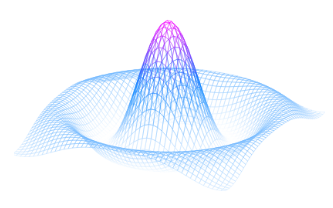
\includegraphics[width=0.4\textwidth]{fig_example.png}
    % Подпись
    \caption{Некоторый график}
    % Метка для ссылки на рисунок
    \label{fig:some_plot}
\end{figure}
\end{verbatim}
%
\begin{figure}[h]
    \centering
    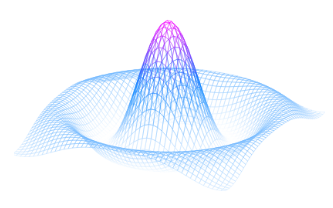
\includegraphics[width=0.4\textwidth]{fig_example.png}
    % Подпись
    \caption{Некоторый график}
    % Метка для ссылки на рисунок
    \label{fig:some_plot}
\end{figure}

Здесь важно помнить, что в преамбуле у нас есть фраза
\begin{verbatim}
    \graphicspath{{\subfix{../images/}}}
\end{verbatim}
задающая папку, в которой хранятся картинки.
Поэтому мы можем указывать в \texttt{includegraphics} только имя файла.

Сослаться всё так же просто.
Вот пример:
\begin{verbatim}
На рисунке~\ref{fig:some_plot} изображена функция ,,сомбреро''.
\end{verbatim}
Отображается как: <<На рисунке~\ref{fig:some_plot} изображена функция ,,сомбреро''.>>

\textbf{
    Помните о том, что перекрёстные ссылки требуют двух компиляций.
}

\textbf{
    И не забывайте про неразрывные пробелы.
    Номера рисунков, таблиц и формул не должны стоять в начале строки без упоминания перед ними, что именно означает цифра.
}

\end{document}
